\documentclass[a4paper,10pt]{scrartcl}

% Hier die Nummer des Blatts und Autoren angeben.
\newcommand{\blatt}{8}
\newcommand{\autor}{Jim Martens}

\usepackage{hci}
\usepackage[utf8]{inputenc}
\usepackage{float}
\usepackage[official]{eurosym}
\usepackage[parfill]{parskip}

\begin{document}
% Seitenkopf mit Informationen
\kopf
\renewcommand{\figurename}{Figure}

\aufgabe{1}

\subsection*{Schlechtes Design}

Das schlechte Design ist die Anordnung und Ausführung des Touchpads des Laptops, auf dem ich diese Zeilen schreibe. Das Touchpad, inklusive der darunter befindlichen Buttons für den linken und den rechten Mausklick, befindet sich zentral bezogen auf die Gesamtbreite des Laptops. 
Das Problem daran ist, dass das ebenfalls in der Tastatur befindliche NumPad eher selten verwendet wird und daher stets eine größere Handbewegung nötig ist, um das Touchpad zu erreichen (Homing, Fitt's Law).

Ein weiteres Problem sind die Mausbuttons, die sich unter dem Touchpad befinden und damit weit abseits der Ruheposition der Hände auf der Tastatur. Für einen Mausklick (links oder rechts) muss daher immer die ganze Hand nach unten bewegt werden (Homing, Fitt's Law).

Desweiteren ist die Qualität der Buttons selber schlecht, sodass bei alltagsmäßigem Gebrauch die Funktionsfähigkeit der Buttons schnell nachlässt und das Klicken über das Touchpad zu erfolgen hat.

\subsection*{Gutes Design}

Das gute Design ist die Maus für meinen Tower-PC. Die Maus hat nicht nur zwei Buttons, sowie ein Mausrad, sondern ist zudem ergonomisch sinnvoll gebaut.
Auf der linken Seite befinden sich eine Einbuchtung, um den Daumen zu parken, sowie zwei kleine vom Daumen bediente Buttons, die bspw. für das Navigieren in der Browserhistorie verwendet werden können.

Die rechte Seite bietet ebenso Platz, um den Ringfinger und kleinen Finger zu parken, sodass die gesamte Bedienung angenehm ist und selbst stundenlange Spielsessions nicht unangenehm auffallen.

\subsection*{Verbesserung}

Im folgenden lassen sich die drei Designskizzen finden. Kurz zusammengefasst werden diese Änderungen vorgenommen:

Die bisherigen Mausbuttons werden in das untere Ende des Touchpads integriert. Zudem gibt es Scollareas in dem Touchpad, sodass einfach mit einem Finger gescrollt werden kann.

Zusätzlich wurden zwei vernünftige Buttons (mit richtigem Widerstand, nicht nur Druckflächen) überhalb des Touchpads eingebaut, sodass diese mit den beiden Daumen bedienbar sind und die Hand nicht mehr für das Klicken bewegt werden muss. Dies vermeidet die Homing-Aktionen komplett, da nur der Daumen bewegt werden muss. Aufgrund der geringeren Distanz ist dies auch nach Fitt's Law vorteilhaft.
Desweiteren wurde ein TrackPoint in die Mitte der mittleren Tastenreihe eingebaut, sodass einfach mit dem Zeigefinger der Mauszeiger bewegt werden kann. Dies ist hier genauso ohne Handbewegung möglich, was nach einer Eingewöhnzeit eine erhebliche Produktivitätserhöhung mit sich bringt, da die Handbewegungen von Tastatur zu Touchpad (Homing-Aktionen) entfallen.

Im Endeffekt muss man die Hände nicht mehr von der Tastatur entfernen und kann somit auch seine Hand- und Armgelenke schonen.

\begin{figure}
	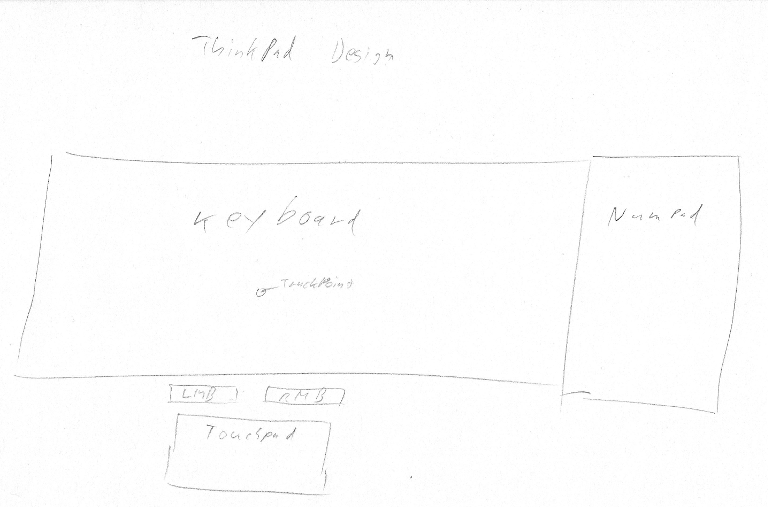
\includegraphics[scale=0.5]{generalDesign_scaled}
	\caption{Allgemeines Design der Verbesserung}
\end{figure}

\begin{figure}
	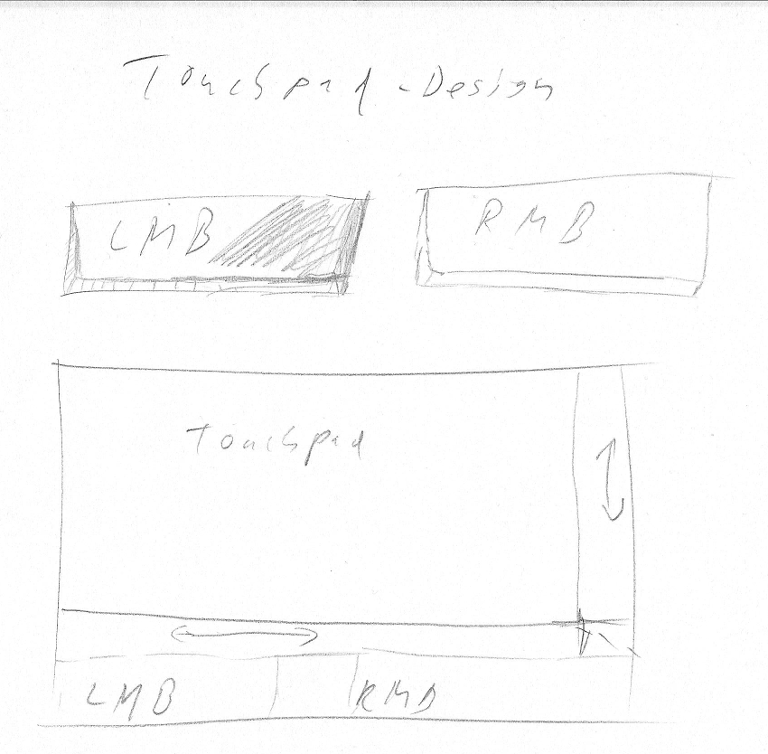
\includegraphics[scale=0.5]{touchpadDesign_scaled}
	\caption{Design des Touchpads in größerem Detail}
\end{figure}

\begin{figure}
	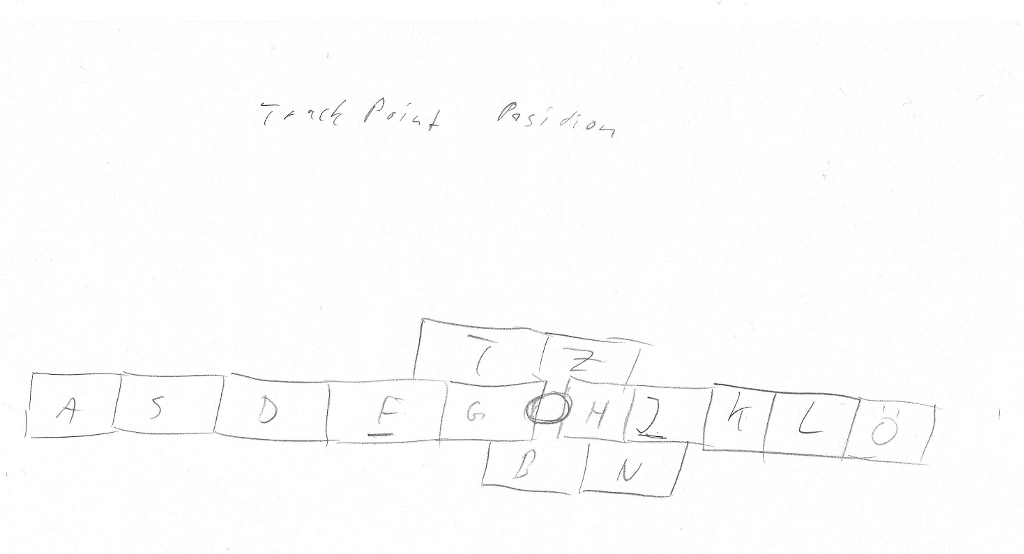
\includegraphics[scale=0.5]{trackPointPosition_scaled}
	\caption{Position des Trackpoints in dem Tastaturlayout}
\end{figure}
\end{document}